%!TEX root = ../main.tex
\chapter{Examples}
\label{chap:examples}

\section{First Example}
\label{chap:first_example}
This is a citation \cite{buch}, this a double citation \cite{buch, buch}.

\subsection{Sub Example}
\label{chap:second_example}

You can reference other chapters or sections by \ref{chap:first_example} 
You can also reference an acronym by \ac{cmyk}


\vspace{5mm}
\begin{figure}[htbp]
	\centering
	\begin{minipage}{0.7\linewidth}
		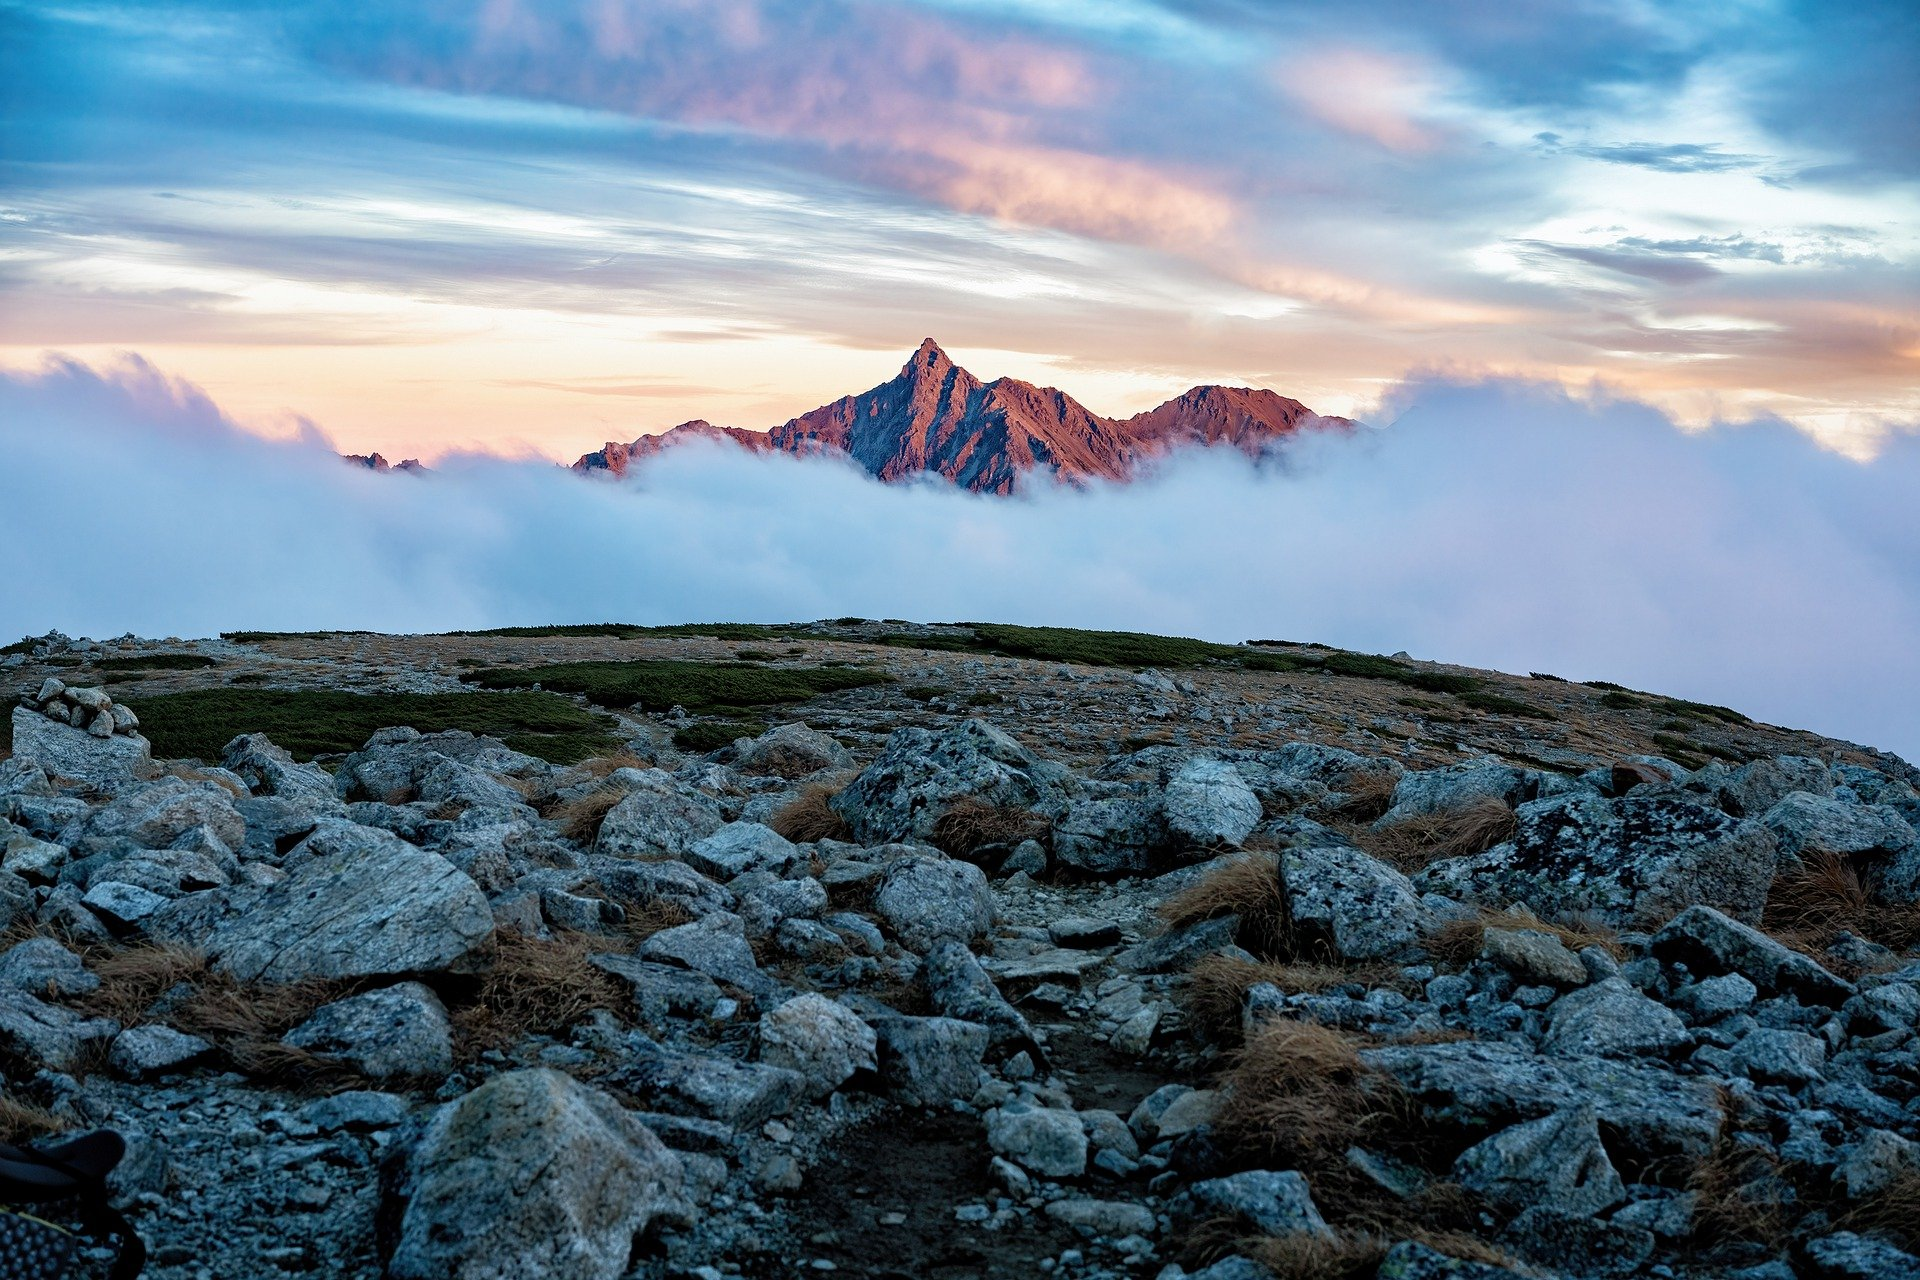
\includegraphics[width=1\linewidth]{landscape}
	\end{minipage}
	\caption{Image caption \cite[S.~5]{buch}}
	\label{img:example_img}
\end{figure}

\subsection{Enumerate}

Enumerate for counted points
\begin{enumerate}
	\item Item 1
	\item Item 2
\end{enumerate}

Use Itemize for bullet points (here also with Header).
\begin{itemize}
	\item \textbf{Header} \\
	Text
	
	\item \textbf{Header} \\
	Text
\end{itemize}

\section{Tables}


\vspace{1em}
\begin{table}[H]
	\centering
	\begin{tabular}{l|cccc}
		\toprule
		\multicolumn{1}{c}{\textbf{Netz}} 
		& \multicolumn{1}{c}{\textbf{Number}}
		& \multicolumn{1}{c}{\textbf{Ratio}}
		& \multicolumn{1}{c}{\textbf{RatioB}} \\
		\midrule
		\multirow{4}{*}{Alpha}
		& 240 & 0\% & 100\% \\
		& 241 & 0\% & 100\% \\
		& 242 & 0\% & 100\% \\
		& 243 & 0\% & 100\% \\
		\cmidrule(lr){1-1}
		\cmidrule(lr){2-4}
		\multirow{4}{*}{Beta}
		& 245 & 1,5\% & 0\% \\
		& 246 & 2,5\% & 0\% \\
		& 247 & 95,5\% & 0\% \\
		& 248 & 0,5\% & 0\% \\
		\bottomrule
	\end{tabular} 
	\captionof{table}[Caption for List of Tables]
    {Caption beneath the table.}
	\label{tab:example_table}
\end{table}


\vspace{1em}
\begin{table}[H]
	\centering
	\begin{tabular}{l|cccc}
		\toprule
		\multicolumn{1}{c}{\textbf{Number}} 
		& \multicolumn{1}{c}{\textbf{Ratio}}
		& \multicolumn{1}{c}{\textbf{RatioB}} 
		& \multicolumn{1}{c}{\textbf{RatioC}}
		& \multicolumn{1}{c}{\textbf{RatioD}}\\
		\midrule
		240 	& 0\% & 100\% & 48\% & 0\% \\
		247 	& 0\% & 100\% & 51\% & 0\% \\
		\bottomrule
	\end{tabular} 
	\captionof{table}[Second Example]
    {Second Table for Examples.}
	\label{tab:vergleich_netz_alpha_vs_beta}
\end{table}